\section{数学细节}\label{sec:2-3}

迄今为止,我们一直比较随意地使用\emph{有效(efficient)}和\emph{可忽略不计(negligible)}这两个术语,而没有给出它们的正式定义:
\begin{itemize}
	\item 我们要求,一个计算性密码要有\emph{有效}的加密和解密算法;
	\item 对于一个语义安全的密码,我们要求任何\emph{有效}对手在攻击游戏 \ref{game:2-1} 中的优势\emph{可忽略不计}。
\end{itemize}
本节的目标是为这些术语提供精确的数学定义。虽然这些定义为密码学作为一门数学学科的研究提供了一个令人满意的理论框架,但我们应该警告读者:
\begin{itemize}
	\item 这些定义相当复杂,需要大量的符号;并且
	\item 这些定义只是非常粗略地模拟了我们对这些术语的直观理解。
\end{itemize}
我们强调,读者可以安全地跳过这一节,而不会在理解上遭受重大损失。在进入正式定义之前,让我们提醒读者,我们在这些定义中试图抓住的东西:
\begin{itemize}
	\item 首先,当我们谈到有效的加密或解密算法时,我们通常指的是一种运行速度非常快的算法,比如以每字节 10 到 100 个时钟周期的速度加密数据。
	\item 其次,当我们说到一个有效对手时,我们通常指的是一个能在某个大的,但仍然可行的时间(和其他计算资源)中运行的算法。通常情况下,我们假设一个试图破解密码学系统的对手愿意花费比密码学系统的用户多得多的资源。因此,10,000 台计算机并行运行 10 年,可以被视为一个坚定的、有耐心的、财力雄厚的对手的可行计算的上限。然而在某些情况下,比如在 \ref{subsec:2-2-4} 小节中的网络轮盘赌的例子中,对手的计算时间可能受到很大的限制。
	\item 第三,当我们说对手的优势可以忽略不计时,我们的意思是它的优势是如此之小,以至于就所有实际目的而言,它都可以被视为等于零。正如我们在网络轮盘赌的例子中所看到的,如果在攻击游戏 \ref{game:2-1} 中,没有一个有效对手拥有超过 $2^{-100}$ 的优势,那么在实践中,就没有一个玩家可以将它在网络轮盘赌中获胜的几率提升到 $2^{-100}$ 以上。
\end{itemize}

尽管我们对\emph{有效}一词的直观理解取决于上下文,但我们的形式化定义不会做这样的区分。事实上,我们将采用计算复杂性理论的习惯,把\emph{有效}算法的概念等同于\emph{(概率性)多项式时间}算法的概念。无论好坏,这都给我们提供了一个独立于任何特定计算模型的具体细节的形式化框架。

\subsection{可忽略不计、超多项式与多项式边界函数}

我们首先定义可忽略不计、超多项式和多项式边界函数的概念。

直观地讲,一个可忽略不计函数 $f:\mathbb{Z}_{\geq0}\to\mathbb{R}$ 是一个不仅在 $n\to\infty$ 时趋近于 $0$,而且趋近于 $0$ 的速度比任何多项式的倒数都要更快的函数。

\begin{definition}\label{def:2-5}
如果对于所有 $c\in\mathbb{R}_{>0}$,都存在 $n_0\in\mathbb{Z}_{\geq 1}$ 使得对于所有的整数 $n\geq n_0$,都有 $|f(n)|<{1}/{n^c}$,我们就称函数 $f:\mathbb{Z}_{\geq1}\to\mathbb{R}$ 是\textbf{可忽略不计的(negligible)}。
\end{definition}

可忽略不计函数的另一种表征,也许更容易理解和使用,如下所示:

\begin{theorem}
当且仅当对于所有 $c>0$,都有:
$$
\lim_{n\to\infty}f(n)n^c=0
$$
时,函数 $f:\mathbb{Z}_{\geq1}\to\mathbb{R}$ 是可忽略不计的。
\end{theorem}

\begin{proof}
留作练习。
\end{proof}

\begin{example}
一些不可忽略函数的例子:
$$
2^{-n},~~2^{-\sqrt{n}},~~n^{-\log n}
$$
一些可忽略函数的例子:
$$
\frac{1}{1000n^4+n^2\log n},~~\frac{1}{n^{100}}
$$
\end{example}

当我们正式定义了``可忽略不计"这个术语后,定义``超多项式"就很容易了。

\begin{definition}
如果 ${1}/{f}$ 可忽略不计,我们就称函数 $f:\mathbb{Z}_{\geq1}\to\mathbb{R}$ 是\textbf{超多项式的(super-poly)}。
\end{definition}

本质上,一个多项式边界函数 $f:\mathbb{Z}_{\geq1}\to\mathbb{R}$ 是一个被某个多项式(绝对值)约束的函数。正式地:

\begin{definition}
如果存在 $c,d\in\mathbb{R}_{>0}$ 使得对于所有整数 $n\geq0$,都有 $|f(n)|\leq n^c+d$,我们就称函数 $f:\mathbb{Z}_{\geq1}\to\mathbb{R}$ 是\textbf{多项式边界的(poly-bounded)}。
\end{definition}

请注意,如果 $f$ 是一个多项式边界函数,那么 ${1}/{f}$ 必然\emph{不是}一个可忽略不计函数。然而,正如下面的例子所说明的那样,请务必注意,不要得出错误的推论。

\begin{example}
定义 $f:\mathbb{Z}_{\geq1}\to\mathbb{R}$,使得对于所有偶数$n$,都有$f(n)={1}/{n}$;对于所有奇数$n$,都有 $f(n)=2^{-n}$。那么$f$不是可忽略不计的,但${1}/{f}$既不是多项式边界的,也不是超多项式的。
\end{example}

\subsection{计算性密码:形式上的问题}

下面,我们讨论形式上的问题。我们首先澄清一个事实:当我们说一个计算性密码 $\mathcal{E}=(E,D)$ 定义在 $(\mathcal{K},\mathcal{M},\mathcal{C})$ 上,其中 $\mathcal{K}$ 是密钥空间,$\mathcal{M}$ 是消息空间,$\mathcal{C}$ 是密文空间,而且每个上述空间都是有限集时,我们并没有说出全部的事实。在数学模型中(尽管在现实世界的系统中并不总是如此),我们将一个密码\emph{族} $\mathcal{E}$ 的密钥、消息和密文空间相关联,其索引为:
\begin{itemize}
	\item 一个\textbf{安全参数(security parameter)}是一个正整数,用$\lambda$表示,和
	\item 一个\textbf{系统参数(system parameter)}是一个比特串,用$\Lambda$表示。
\end{itemize}
因此,现在 $\mathcal{K},\mathcal{M},\mathcal{C}$ 不再单是三个有限集,而是三个有限集族:
$$
\{\mathcal{K}_{\lambda,\Lambda}\}_{\lambda,\Lambda},\quad
\{\mathcal{M}_{\lambda,\Lambda}\}_{\lambda,\Lambda},\quad
\{\mathcal{C}_{\lambda,\Lambda}\}_{\lambda,\Lambda}
$$
在本定义中,我们将其视为比特串的集合(可以通过一些规范的编码函数来表示数学对象)。

我们的想法是,当密码 $\mathcal{E}$ 被部署时,安全参数 $\lambda$ 会被固定为某个值。一般来说,$\lambda$ 的值越大,意味着安全水平就越高(即对拥有更多计算资源的对手的具备抵抗力),但也意味着更大的密钥长度,以及更慢的加解密速度。因此,安全参数就像一个我们可以转动的``拨盘",用于在安全和效率之间进行权衡。

一旦选定了 $\lambda$,系统参数$\Lambda$就会用一种特定于密码的算法生成。我们的想法是,系统参数 $\Lambda$(连同$\lambda$)给出了一个固定密码实例的详细描述,即:
$$
(\mathcal{K},\mathcal{M},\mathcal{C})=(\mathcal{K}_{\lambda,\Lambda},\;\mathcal{M}_{\lambda,\Lambda},\;\mathcal{C}_{\lambda,\Lambda})
$$
这一固定的实例可能会被部署在一个更大的系统中,并被多方使用,其中的$\lambda$和$\Lambda$的值都是公开的,(包括对手在内的)每个人都能知道。

\begin{example}\label{exmp:2-12}
考虑例 \ref{exmp:2-4} 中讨论的加性一次性密码本。这个密码使用了一个模数$n$作为描述。要部署这样一个密码,需要生成一个合适的模数 $n$,并将其公开(有时甚至会将其直接``硬编码"到实现密码的程序里)。模数 $n$ 就是这个密码的系统参数。安全参数的每个特定值决定了$n$的长度,以比特为单位。$n$ 本身可能由某些算法产生,这些算法可能是概率性的,其输出分布可能取决于预期的应用场景。例如,在某些场景下我们希望 $n$ 是一个素数。
\end{example}

在进一步讨论之前,我们需要先定义有效算法的概念。为了这个目的,我们将只考虑以安全参数$\lambda$和总长度由$\lambda$的多项式约束的其他参数作为输入的算法$A$。基本上,我们想说 $A$ 的运行时间是以 $\lambda$ 的多项式为界的,但如果 $A$ 是概率性的,情况将更加复杂:

\begin{definition}[有效算法]
令 $A$ 是一个算法(可能是概率性的),它以一个安全参数 $\lambda\in\mathbb{Z}_{\geq1}$,以及其他被编码成的一个比特串 $x\in\{0,1\}^{\leq p(\lambda)}$ 的若干参数作为输入,其中 $p(\lambda)$ 是 $\lambda$ 的一个固定的多项式。如果存在一个多项式边界函数 $t$ 和一个可忽略不计函数 $\epsilon$,使得对于所有的 $\lambda\in\mathbb{Z}_{\geq1}$ 和所有的 $x\in\{0,1\}^{\leq p(\lambda)}$,算法 $A$ 在输入 $(\lambda,x)$ 上的运行时间超过 $t(\lambda)$ 的概率最多为 $\epsilon(\lambda)$,我们就称 $A$ 为一个\textbf{有效算法(efficient algorithm)}。
\end{definition}

我们强调,上述定义中的概率是针对$A$的抛硬币而言的:对概率的这个约束必须对所有可能的输入$x$都成立。
\footnote{
\label{foot:2-1}
我们不坚持概率性算法在指定的时间范围内以$1$的概率停止,这样能给我们一点``回旋的余地",使得我们能够轻松地执行某些类型的随机抽样程序,这些程序没有\emph{先验的}运行时间限制,但不太可能运行非常长的时间(例如扔硬币直到出现正面)。另一种方法是约束\emph{预期的}运行时间,但由于技术原因,这被证明是有问题的。

请注意,这个有效算法的定义并不要求该算法在所有输入上都以$1$的概率停止。一个以$2^{-\lambda}$的概率进入无限循环的算法也可以满足这个定义,即使它不是以$1$的概率停止。这些问题是相当传统的。一般来说,我们只考虑在所有输入上都能以 $1$ 的概率停止的算法:这可以更自然地被看作是对算法的输出分布的要求,而不是对其运行时间的要求。
}

下面是一个正式定义,它抓住了由安全参数和系统参数进行参数化的系统的基本要求,并引入了更多的术语。在下面的定义中,我们用 ${\rm Supp}(P(\lambda))$ 来指代分布 $P(\lambda)$ 的\textbf{支持(support)},即算法 $P$ 在输入 $\lambda$ 上所有可能输出的集合。

\begin{definition}\label{def:2-9}
一个\textbf{系统参数化(system parameterization)}是一个有效概率性算法 $P$,它以一个给定的安全参数 $\lambda\in\mathbb{Z}_{\geq1}$为输入,输出一个比特串 $\Lambda$,称为\textbf{系统参数},其长度总是以 $\lambda$ 的一个多项式为界。我们还定义以下术语:
\begin{itemize}
	\item 一个由比特串的有限集 $\mathbf{S}=\{\mathcal{S}_{\lambda,\Lambda}\}_{\lambda,\Lambda}$ 组成的集合,其中 $\lambda$在$\mathbb{Z}_{\geq1}$上运行,$\Lambda$在${\rm Supp}(P(\lambda))$上运行,当每个集合 $\mathcal{S}_{\lambda,\Lambda}$ 中的所有比特串的长度都被 $\lambda$ 的某个多项式 $p$ 约束,我们就称 $\mathbf{S}$ 为\textbf{具有系统参数化 $P$ 的空间族(family of spaces with system parameterization $P$)}。
	\item 如果存在一个有效确定性算法,在输入 $\lambda\in\mathbb{Z}_{\geq1}$,$\Lambda\in{\rm Supp}(P(\lambda))$,$s\in\{0,1\}^{\leq p(\lambda)}$ 上能够确定 $s\in\mathcal{S}_{\lambda,\Lambda}$ 是否成立,就称 $\mathbf{S}$ 是\textbf{可有效识别的(efficiently recognizable)}。
	\item 如果存在一个有效概率性算法,在输入 $\lambda\in\mathbb{Z}_{\geq1}$,$\Lambda\in{\rm Supp}(P(\lambda))$ 上能够输出一个均匀分布在 $\mathcal{S}_{\lambda,\Lambda}$ 上的元素,就称 $\mathbf{S}$ 是\textbf{可有效采样的(efficiently sampleable)}。
	\item 如果存在一个有效确定性算法,在输入 $\lambda\in\mathbb{Z}_{\geq1}$,$\Lambda\in{\rm Supp}(P(\lambda))$,$s\in\mathcal{S}_{\lambda,\Lambda}$ 上能够输出一个非负整数,称为 $s$ 的\textbf{长度},则称 $\mathbf{S}$ \textbf{有一个有效长度函数(has an effective length function)}。
\end{itemize}
\end{definition}

现在,我们就可以给出计算性密码完整且正式的定义:

\begin{definition}[计算性密码]\label{def:2-10}
一个\textbf{计算性密码}由一对算法 $E$ 和 $D$,以及三个具有系统参数化 $P$ 的空间族:
$$
\mathbf{K}=\{\mathcal{K}_{\lambda,\Lambda}\}_{\lambda,\Lambda},\quad
\mathbf{M}=\{\mathcal{M}_{\lambda,\Lambda}\}_{\lambda,\Lambda},\quad
\mathbf{C}=\{\mathcal{C}_{\lambda,\Lambda}\}_{\lambda,\Lambda}
$$
组成,满足:
\begin{enumerate}
	\item $\mathbf{K}$,$\mathbf{M}$和$\mathbf{C}$都是可有效识别的。
	\item $\mathbf{K}$是可有效采样的。
	\item $\mathbf{M}$有一个有效长度函数。
	\item 算法 $E$ 是一个有效概率性算法,它接受 $\lambda,\Lambda,k,m$ 作为输入,其中 $\lambda\in\mathbb{Z}_{\geq1}$,$\Lambda\in{\rm Supp}(P(\lambda))$,$k\in\mathcal{K}_{\lambda,\Lambda}$,$m\in\mathcal{M}_{\lambda,\Lambda}$,总是输出一个 $\mathcal{C}_{\lambda,\Lambda}$ 中的元素。
	\item 算法 $D$ 是一个有效确定性算法,它接受 $\lambda,\Lambda,k,c$ 作为输入,其中 $\lambda\in\mathbb{Z}_{\geq1}$,$\Lambda\in{\rm Supp}(P(\lambda))$,$k\in\mathcal{K}_{\lambda,\Lambda}$,$c\in\mathcal{C}_{\lambda,\Lambda}$,输出一个 $\mathcal{M}_{\lambda,\Lambda}$ 中的元素,或一个特殊符号 $\mathsf{reject}\notin\mathcal{M}_{\lambda,\Lambda}$。
	\item 对于所有的 $\lambda,\Lambda,k,m,c$,其中$\lambda\in\mathbb{Z}_{\geq1}$,$\Lambda\in{\rm Supp}(P(\lambda))$,$k\in\mathcal{K}_{\lambda,\Lambda}$,$m\in\mathcal{M}_{\lambda,\Lambda}$,如果 $c\in{\rm Supp}(E(\lambda,\Lambda;k,m))$,必有$D(\lambda,\Lambda;k,c)=m$。
\end{enumerate}
\end{definition}


注意,在上述定义中,加密和解密算法接受 $\lambda$ 和 $\Lambda$ 作为辅助输入。为了与 \ref{subsec:2-2-1} 小节中所介绍的符号保持一定的一致性,我们把它们写成 $E(\lambda,\Lambda;\cdots)$ 和 $D(\lambda,\Lambda;\cdots)$。

\begin{example}
考虑加性一次性密码本(见例 \ref{exmp:2-12})。在我们的正式框架中,安全参数 $\lambda$ 决定了模数 $n$ 的比特长度 $L(\lambda)$,也就是系统参数。系统参数生成算法将 $\lambda$ 作为输入,生成长度为 $L(\lambda)$ 的模数 $n$。函数 $L(\cdot)$ 应该是一个多项式边界函数。有了这个假设,很明显,系统参数生成算法满足对它的要求。对密钥、消息和密文空间的要求也得到了满足:
\begin{enumerate}
	\item 这些空间中的元素具有多项式边界长度:这是因为我们假设 $L(\cdot)$ 是一个多项式边界函数。
	\item 密钥空间是可有效采样的:只需选择 $k\overset{\rm R}\leftarrow\{0,\dots,n−1\}$。
	\item 密钥、信息和密文空间都是可有效识别的:只需测试一个比特串 $s$ 是否是 $0$ 和 $n-1$ 之间的某个整数的二进制编码即可。
	\item 消息空间有一个有效长度函数:只需输出(比如) $0$ 即可。
\end{enumerate}
\end{example}

我们注意到,有些密码(例如一次性密码本)可能不需要系统参数。在这种情况下,我们可以假装系统参数是空字符串。我们还注意到,有些密码也并没有真正的安全参数;事实上,很多行业标准的密码根本就是现成的,有一个固定的密钥大小,没有可以调整的安全参数。这根本就是理论与实践的不匹配,但事实就是如此。

这就完成了我们对计算性密码的正式数学描述,并包含所有的细节。
\footnote{
请注意,\ref{subsec:2-2-1} 小节中对香农密码的定义保持不变。在\ref{subsec:2-2-1} 小节末尾提出的``任何确定性计算性密码也是一个香农密码"的说法需要一个更恰当的解释:对于每个$\lambda$和$\Lambda$,我们得到一个定义在$(\mathcal{K}_{\lambda,\Lambda},\mathcal{M}_{\lambda,\Lambda},\mathcal{C}_{\lambda,\Lambda})$上的香农密码。
}
希望读者能够理解,虽然这些形式化的东西可以让我们给出数学上的精确和有意义的陈述,但它们并不是很有启发性,而且大多是为了掩盖真正发生的事情。因此,在正文中,我们将继续使用 \ref{subsec:2-2-1} 小节的简化术语和符号来讨论密码,但需要理解,在本节讨论的形式化框架中,所有的陈述都有适当而自然的解释。这会是一个在接下来的章节中反复出现的模式:我们将主要使用简化的术语讨论各种类型的密码方案,而不讨论安全参数和系统参数。这些数学细节会在单独的一小节中讨论,一般会遵循这里建立的相同的一般模式。

\subsection{有效对手和攻击游戏}

在定义语义安全的概念时,我们必须定义所谓的\emph{有效对手 (efficient adversary)}是什么意思。由于这个概念将在本书中被广泛使用,我们要在这里提出一个更一般的框架。

对于任何类型的加密方案,我们都需要使用一个攻击游戏来定义其安全性,这个攻击游戏通常在一个对手 $\mathcal{A}$ 和它的挑战者之间进行。$\mathcal{A}$ 遵循一个任意的协议,而挑战者遵循一个简单且固定的协议,该协议由所讨论的密码方案及其安全概念所决定。此外,对手和挑战者都将一个共同的安全参数 $\lambda$ 作为输入,挑战者在游戏开始时会计算出一个相应的系统参数 $\Lambda$,并将其发送给对手 $\mathcal{A}$。

为了对这些类型的交互进行建模,我们引入\textbf{交互式机器 (interactive machine)}的概念。在这样的机器 $M$ 启动之前,它总是会得到写在一个特殊缓冲区中的安全参数 $\lambda$,并且其内部状态的其他部分会被初始化为某个默认值。机器 $M$ 还有两个特殊的缓冲区:一个\emph{传入消息缓冲区(incoming message buffer)}和一个\emph{传出消息缓冲区(outcoming message buffer)}。机器 $M$ 可以被多次调用:当$M$ 的外部环境向 $M$ 的传入消息缓冲区写入一个字符串时,新的调用就开始了;$M$读取该消息,进行一些计算,更新其内部状态,并在其传出消息缓冲区上写入一个字符串,最后结束调用,将传出消息交给外部环境。因此,$M$ 通过一个简单的消息传递系统与它的环境进行交互。我们假设 $M$ 可以在它的最后一个传出消息中嵌入一些信号,以此来表示它已经停止,随后 $M$ 会忽略任何调用它的尝试。

我们假设传入和传出机器 $M$ 的消息都被限制为\emph{恒定的长度}。这其实并不是一个真正的限制,因为我们总是可以通过发送许多较短的消息来模拟一个长消息的传输。然而,做出这样的限制可以简化一些技术问题。从现在开始,我们对对手和其他任何类型的交互式机器都施加这种长度限制。

对于任何给定的环境,我们可以通过计算 $M$ 在所有调用中执行的步骤的数量来衡量 $M$ 的\textbf{总运行时间 (total running time)}。这个运行时间不仅取决于 $M$ 和它的随机选择,还取决于 $M$ 运行的环境。
\footnote{
与脚注 \ref{foot:2-1} 的讨论类似,我们对有效交互式机器的定义并不要求它在所有环境下都以 $1$ 的概率停机。这也是一个传统问题,但它将是我们考虑的任何机器的一个隐含要求。
}

\begin{definition}[有效交互式机器]
如果存在一个多项式边界函数 $t$ 和一个可忽略不计函数 $\epsilon$,使得对于所有环境(甚至不仅是计算上有边界的环境),$M$ 的总运行时间超过 $t(\lambda)$ 的概率最多为 $\epsilon(\lambda)$,我们就称 $M$ 是一个\textbf{有效交互式机器 (efficient interactive machine)}。
\end{definition}


自然而然地,我们可以将对手建模为一个交互式机器。一个\textbf{有效对手 (efficient adversary)}就是一个有效交互式机器。

我们可以将两个交互式机器连接在一起,比如使用 $M'$ 和 $M$ 构建一个新的交互式机器 $M''=\langle M',M\rangle$。从环境到 $M''$ 的消息总是会被转发到 $M'$。机器 $M'$ 可以向环境发送消息,也可以向 $M$ 发送消息;在后一种情况下,$M$ 发送的输出消息会被发送到 $M'$。我们假设,如果 $M$ 停机,那么 $M'$ 就不会再向它发送任何消息。

因此,当 $M''$ 被调用时,其传入的消息会被转发到 $M'$,然后 $M'$ 和 $M$ 可能会交互若干次,然后,当 $M'$ 向环境发送消息时,$M''$ 的调用就结束了。我们称 $M'$ 为``开放的"机器(即它与外界交互),$M$ 为``封闭的"机器(即它只与 $M'$ 交互)。

\vspace{8pt}

自然,我们可以通过将两台这样的机器连接在一起来模拟挑战者和对手的交互,如上所述:挑战者为开放的机器,而对手为封闭的机器。

在我们的安全归约中,我们通常会展示如何使用能够破坏某个系统的对手 $\mathcal{A}$ 来构建能够破坏其他系统的对手 $\mathcal{B}$。我们想要的基本属性是,如果 $\mathcal{A}$ 是有效的,那么 $\mathcal{B}$ 也是有效的。然而,我们的归约几乎总是一种非常特殊的形式,即 $\mathcal{B}$ 是 $\mathcal{A}$ 的一个包装器,它由位于 $\mathcal{B}$ 的挑战者与 $\mathcal{A}$ 的单个运行实例之间的某个简单而有效的``接口层"组成。

理想情况下,我们希望接口层的计算复杂度不依赖于 $\mathcal{A}$ 的计算复杂度;然而,某种程度的依赖性是不可避免的:$\mathcal{A}$ 向其挑战者进行的查询越多,接口层就必须执行越多的工作,但这种工作应该只是依赖于这种查询的数量,而不依赖于 $\mathcal{A}$ 的运行时间。

为了形式定义这一点,我们将 $\mathcal{B}$ 构建为一个组合式机器 $\langle M',M\rangle$,其中 $M'$ 代表接口层(即``开放的"机器),$M$ 代表 $\mathcal{A}$ 的实例(即``封闭的“机器)。这就导出了下面的定义。

\begin{definition}[基本包装器]\label{def:2-12}
如果存在一个多项式边界函数 $t$ 和一个可忽略不计函数 $\epsilon$,使得对于所有的机器 $M$(不必是计算上有界的),当我们在一个任意的环境(同样,不必是计算上有界的)中执行组合式机器 $\langle M',M\rangle$ 时,下述属性成立:
\begin{quote}
在组合式机器 $\langle M',M\rangle$ 执行的每一点上,如果 $I$ 是 $M'$ 和 $M$ 之间截至该点的交互次数,$T$ 是 $M'$ 截至该点的总运行时间,则 $T>t(\lambda+I)$ 的概率最大为 $\epsilon(λ)$。
\end{quote}
我们就称交互式机器 $M'$ 为一个\textbf{有效接口 (efficient interface)}。如果 $M'$ 是一个有效接口,而 $M$ 是任何机器,我们都称 $\langle M',M\rangle$ 是\textbf{一个围绕 $M$ 的基本包装器 (an elementary wrapper around $M$)}。
\end{definition}

因此,当对手 $\mathcal{B}$ 能够像上面那样被结构化为一个与 $\mathcal{A}$ 交互的有效接口时,我们就称 $\mathcal{B}$ 是一个围绕 $\mathcal{A}$ 的基本包装器。我们的定义被设计成很适合协同工作的形式,其突出的属性是:
\begin{itemize}
	\item 如果 $\mathcal{B}$ 是一个围绕 $\mathcal{A}$ 的基本包装器,而 $\mathcal{A}$ 是有效的,那么 $\mathcal{B}$ 也是有效的。
	\item 如果 $\mathcal{C}$ 是一个围绕 $\mathcal{B}$ 的基本包装器,$\mathcal{B}$ 是一个围绕 $\mathcal{A}$ 的基本包装器,那么 $\mathcal{C}$ 是一个围绕 $\mathcal{A}$ 的基本包装器。
\end{itemize}

还要注意的是,在我们的攻击游戏中,挑战者通常满足我们对有效接口的定义。对于这样的挑战者和任何一个有效对手 $\mathcal{A}$,我们可以将它们的整个交互看作是一个单一的有效机器的交互。

\begin{snote}[查询有界对手。]
在我们到目前为止所介绍的所有攻击游戏中,对手都只会发起固定数量的查询。在后面的章节中,我们将看到对手 $\mathcal{A}$ 被允许进行多次查询,而且它的查询次数没有先验约束。如果 $\mathcal{A}$ 是有效的,那么查询的次数会被某个多项式边界值 $Q$ 所约束(至少以几乎可忽略不计的概率)。在证明这种攻击游戏的安全性时,为了设计一个围绕 $\mathcal{A}$ 的基本包装器 $\mathcal{B}$,我们通常会\emph{预先}向 $\mathcal{B}$ 告知 $\mathcal{A}$ 最终会进行的查询次数的上界 $Q$。为了应用形式化框架,我们可以让 $\mathcal{A}$ 在一开始就发送一连串的 $Q$ 个特殊消息,来向 $\mathcal{B}$ ``通知"该查询次数上界。如果这样做,那么 $\mathcal{B}$ 不仅可以在其逻辑中使用 $Q$ 值,而且还可以在不违反定义 \ref{def:2-12} 中的时间约束的情况下,以取决于 $Q$ 的时间运行。这就使得 $\mathcal{B}$ 可以初始化一些大小可能依赖于 $Q$ 的数据结构。当然,所有这些都只是一个理论上的``hack",用来绕过那些本来就过于严苛的技术约束,因此不应该太认真。我们在接下来的章节中都不会再明确说明这种``通知机制"。
\end{snote}


\subsection{语义安全性:形式上的问题}

在定义任何类型的安全性时,我们把对手在攻击游戏中的优势定义为一个函数 ${\rm Adv}(\lambda)$。它的值由攻击游戏中某些事件发生的概率来决定:对于 $\lambda$ 的每个值,我们都能得到一个不同的概率空间,它由挑战者的随机选择和对手的随机选择共同决定。安全性意味着,对于每个有效对手,函数 ${\rm Adv}(\cdot)$ 的值都可忽略不计。

下面我们谈谈密码的语义安全性。在攻击游戏 \ref{game:2-1} 中,我们定义了 ${\rm SS\mathsf{adv}}[\mathcal{A},\mathcal{E}]$ 这个值。这个值实际上是安全参数 $\lambda$ 的一个函数。对定义 \ref{def:2-2} 的正确解释是,如果对于所有有效对手 $\mathcal{A}$(如上所述,它被建模为一个交互式机器)来说,安全参数 $\lambda$ 的函数 ${\rm SS\mathsf{adv}}[\mathcal{A},\mathcal{E}]$ 都可忽略不计(如定义 \ref{def:2-5} 所定义的那样),则 $\mathcal{E}$ 是安全的。回顾一下,挑战者和对手都接受 $\lambda$ 作为共同的输入。交互从挑战者开始,它将系统参数发送给对手。随后,对手将它的查询发送给挑战者,其中包含两条明文,而挑战者会用一条密文作为应答。最后,对手会输出一个比特(严格来说,在我们的形式化机器的模型中,这个``输出"是发送给挑战者的一条消息,然后挑战者停机)。${\rm SS\mathsf{adv}}[\mathcal{A},\mathcal{E}]$ 的值由挑战者的随机选择(包括系统参数的选择)和对手的随机选择共同决定。图 \ref{fig:2-6} 展示了攻击游戏 \ref{game:2-1} 的全貌。

\begin{figure}
  \centering
  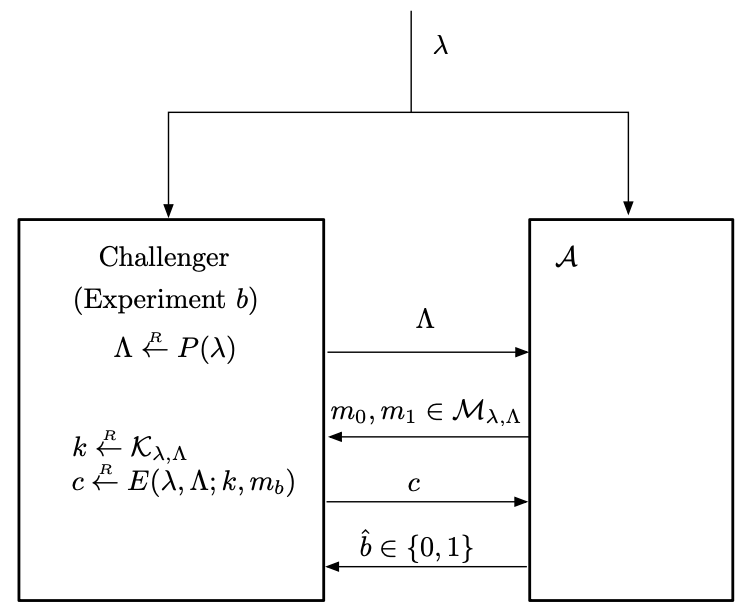
\includegraphics[width=0.5\linewidth]{figures/chapter2/fig6.png}
  \caption{攻击游戏 \ref{game:2-1} 的完整详细版本}
  \label{fig:2-6}
\end{figure}

此外,在攻击游戏 \ref{game:2-1} 中,我们要求对手给出的两条消息具有相同的长度,这意味着定义 \ref{def:2-10} 第 3 部分给出的长度函数在两条消息上评估为相同的值。

根据这个形式上的定义,我们也可以讨论一下密码 $\mathcal{E}$ 的不安全到底意味着什么。这意味着存在一个有效对手 $\mathcal{A}$,使得 ${\rm SS\mathsf{adv}}[\mathcal{A},\mathcal{E}]$ 是一个 $\lambda$ 的不可忽略不计函数。即对于某个 $c>0$ 和无限多个安全参数 $\lambda$ 的取值,有 ${\rm SS\mathsf{adv}}[\mathcal{A},\mathcal{E}]\geq{1}/{\lambda^c}$ 成立。所以,不安全性并不意味着对于所有的安全参数 $\lambda$,对手 $\mathcal{A}$ 都能``攻破"密码 $\mathcal{E}$,而只是对于无限多个 $\lambda$,对手 $\mathcal{A}$ 能攻破密码 $\mathcal{E}$。

在正文中,我们一般会忽略安全参数、系统参数等。但读者需要明白,所有这些``简写"的背后都存在一个相应的精确的、形式化的数学表达。特别地,我们经常会称某个值 $v$ 是可忽略不计的(多项式边界的),这实际上意味着 $v$ 是安全参数的一个可忽略不计(多项式边界)函数。